\documentclass[11pt,a4paper]{article}

\usepackage[margin=2.2cm]{geometry}
\usepackage{graphicx}
\usepackage{booktabs}
\usepackage{xcolor}
\usepackage{hyperref}
\usepackage{caption}
\usepackage[labelfont=bf,labelsep=period]{caption}

\definecolor{blue}{HTML}{2A78D6}
\definecolor{orange}{HTML}{EB6834}
\definecolor{dark}{HTML}{0B0B0B}
\definecolor{gray}{HTML}{898781}
\definecolor{green}{HTML}{0CA30C}

\hypersetup{colorlinks=true,linkcolor=blue,urlcolor=blue,citecolor=blue}

\begin{document}

\title{\textbf{Classic vs.\ Affine DDPNM: Error and Cost across 3D Geometries}}
\author{}
\date{\today}
\maketitle

\section{Summary}

We compare the classic one-constant-normal-traction-per-interface
\textbf{Classic-DDPNM} against the nine-mode
($\{1,s,t\}\times\{n,t_1,t_2\}$) \textbf{Affine-DDPNM} on three
three-dimensional geometries, all sharing the identical tetrahedral mesh
with their monolithic Taylor--Hood P2--P1 reference solution.

\begin{figure}[htbp]
  \centering
  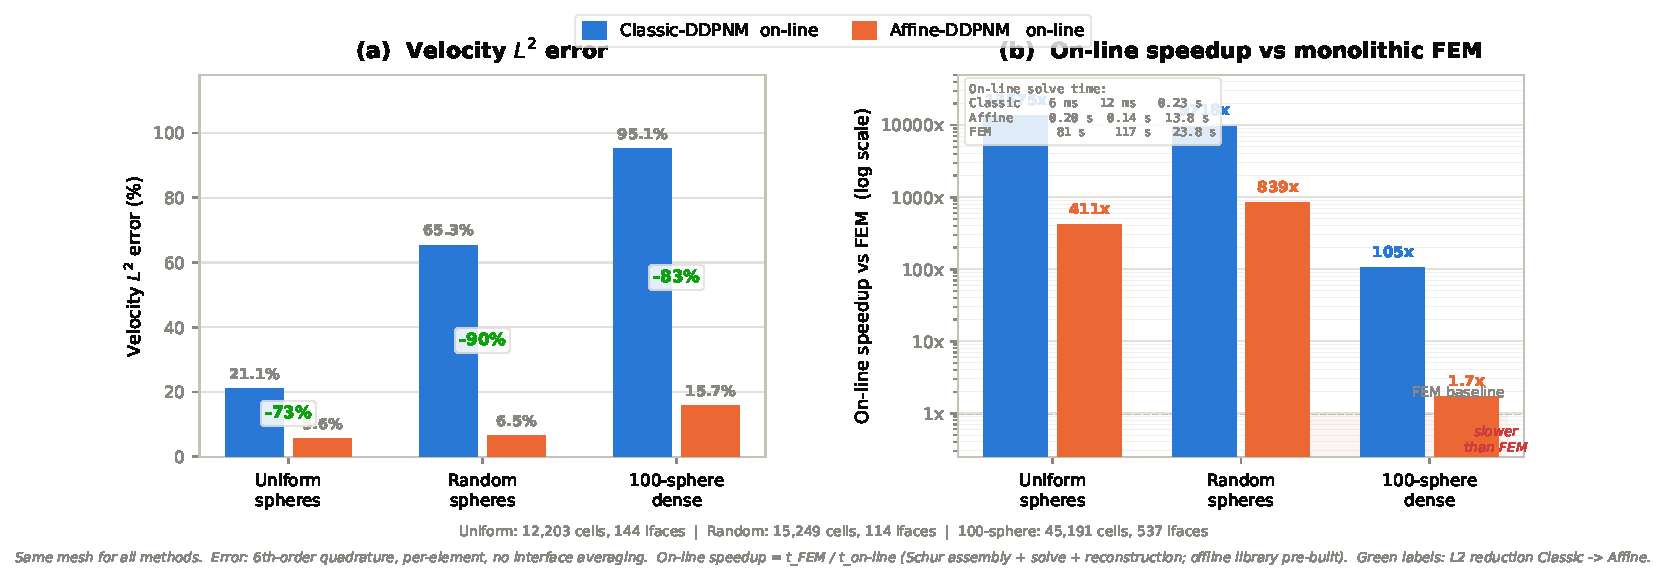
\includegraphics[width=\textwidth]{fig_classic_vs_affine.pdf}
  \caption{Comparison across three 3D geometries.
    (a)~Velocity $L^2$ error relative to monolithic FEM; green labels show
    the relative reduction Classic $\to$ Affine.
    (b)~Wall time breakdown: solid fill = offline local-response library;
    hatched overlay = on-line Schur assembly $+$ solve $+$ reconstruction.
    Grey bars = monolithic FEM reference time.
    Annotated on-line speedup = $t_{\text{FEM}} \,/\, t_{\text{on-line}}$,
    i.e.\ the per-boundary-condition advantage once the offline library is built.
    The 100-sphere benchmark uses a standard Voronoi partition; polydisperse
    radii ($r_{\max}-r_{\min}=0.041 > \text{gap}/2$) cause Voronoi faces
    to cut through spheres, inflating both methods' errors.}
  \label{fig:main}
\end{figure}

\section{Results}

\begin{table}[htbp]
  \centering
  \caption{Same-mesh error: Classic vs.\ Affine DDPNM.}
  \label{tab:errors}
  \small
  \begin{tabular}{@{}lcccccccc@{}}
    \toprule
    & \multicolumn{4}{c}{\textbf{Classic-DDPNM}} & \multicolumn{4}{c}{\textbf{Affine-DDPNM}} \\
    \cmidrule(lr){2-5} \cmidrule(lr){6-9}
    Geometry & $L^2(u)$ & $H^1(u)$ & $L^2(p)$ & Flux & $L^2(u)$ & $H^1(u)$ & $L^2(p)$ & Flux \\
    \midrule
    Uniform (27)    & 21.1\% & 44.8\% & 3.2\% & 16.5\% & 5.6\% & 21.6\% & 2.2\% & 0.3\% \\
    Random (27)     & 65.3\% & 85.9\% & 10.3\% & 72.7\% & 6.5\% & 17.6\% & 2.0\% & 2.7\% \\
    100-sphere      & 95.1\% & 115.6\% & 11.2\% & 132.2\% & 15.7\% & 30.2\% & 2.5\% & 8.7\% \\
    \bottomrule
  \end{tabular}
\end{table}

\begin{table}[htbp]
  \centering
  \caption{Computational cost: offline (local response library),
    on-line (Schur assembly $+$ solve $+$ reconstruction), and on-line speedup
    vs.\ monolithic FEM.  First-solve = offline $+$ on-line.}
  \label{tab:cost}
  \small
  \begin{tabular}{@{}lrrrrrrr@{}}
    \toprule
    & \multicolumn{3}{c}{\textbf{Classic-DDPNM}} & \multicolumn{3}{c}{\textbf{Affine-DDPNM}} & \\
    \cmidrule(lr){2-4} \cmidrule(lr){5-7}
    Geometry & Offline & On-line & On-line $\times$FEM & Offline & On-line & On-line $\times$FEM & FEM \\
    \midrule
    Uniform    & 11.2\,s & 6\,ms   & \textbf{13\,600}$\times$ & 13.7\,s & 0.20\,s  & \textbf{410}$\times$ & 81.4\,s \\
    Random     & 12.2\,s & 12\,ms  & \textbf{9\,700}$\times$ & 15.1\,s & 0.14\,s  & \textbf{840}$\times$ & 116.6\,s \\
    100-sphere & 67.7\,s & 0.23\,s & \textbf{105}$\times$   & 89.2\,s & 13.8\,s  & \textbf{1.7}$\times$  & 23.8\,s \\
    \bottomrule
  \end{tabular}
\end{table}

\section{Key findings}

\begin{enumerate}
  \item \textbf{Affine-DDPNM reduces velocity $L^2$ error by 73--90\%}
    across all geometries compared to Classic-DDPNM, with only a
    23--51\% increase in first-solve cost. The nine-mode interface
    space $\{1,s,t\}\times\{n,t_1,t_2\}$ captures in-plane linear
    variations that the single constant-normal mode cannot.

  \item \textbf{Classic 3D DDPNM degrades severely on non-uniform
    geometries.}  Classic velocity $L^2$ error grows from 21\% on
    regular spheres to 65\% on random spheres and 95\% on the dense
    100-sphere packing.  Affine-DDPNM remains at 5.6--15.7\%, with
    the 15.7\% on the 100-sphere case dominated by the underlying
    Voronoi partition error (faces cutting through spheres where
    $r_{\max}-r_{\min} > \text{gap}/2$), not by the interface basis.

  \item \textbf{On-line speedup is massive and persistent.}
    Classic on-line solves ($\le 0.23$\,s) are 105--13\,600$\times$ faster
    than monolithic FEM; Affine on-line solves ($\le 14$\,s) are
    1.7--840$\times$ faster.  The on-line cost is the per-boundary-condition
    cost once the offline library is built---this is where DDPNM's
    multi-query advantage lives.

  \item \textbf{First-solve speedup depends on FEM/offline ratio.}
    Where FEM is expensive (81--117\,s on uniform/random meshes),
    first-solve achieves 5.9--9.6$\times$ speedup.  Where FEM is cheap
    (23.8\,s on the 45K-cell 100-sphere mesh) and offline is heavy
    (68--103\,s, 100 pores $\times$ SuperLU per pore), first-solve is
    slower than FEM.  This is not a failure of DDPNM---it is a mesh-size
    crossover effect: offline cost is a fixed entry fee that amortises
    as the mesh (and FEM cost) grows.

  \item \textbf{The 100-sphere benchmark identifies the next
    bottleneck: partition geometry.}  Polydisperse packings require
    weighted (power) Voronoi partitions to keep interfaces at true
    saddle points.  Standard Voronoi faces cutting through spheres
    inflate both methods' errors; the residual 15.7\% Affine error
    is primarily a partition-model error, not a basis error.
\end{enumerate}

\section*{Mesh specifications}

\begin{itemize}
  \setlength\itemsep{0pt}
  \item \textbf{Uniform}: unit cube $-$ $3\times3\times3$ equal spheres ($r=0.105$),
    64 maximal-ball subdomains, 144 saddle interfaces, 12,203 tetrahedra,
    63,955 FEM DOFs.
  \item \textbf{Random}: unit cube $-$ 27 random spheres (seed 20260804),
    27 Voronoi subdomains, 114 planar Voronoi interfaces, 15,249 tetrahedra,
    75,954 FEM DOFs.
  \item \textbf{100-sphere}: unit cube $-$ 100 polydisperse spheres
    ($r\in[0.055,0.097]$, porosity 85.6\%, seed 20260806),
    100 Voronoi subdomains, 537 interfaces, 45,191 tetrahedra.
\end{itemize}

\end{document}
